\documentclass{beamer} 
\usepackage{amsmath,amsthm}
\usepackage{graphicx,microtype,parskip}
\usepackage{caption,subcaption,multirow}
\usepackage{attrib}

\frenchspacing

\usetheme{default}
\usecolortheme{whale}

\setbeamertemplate{navigation symbols}{}

\setbeamercolor{title}{fg=blue,bg=white}

\setbeamercolor{block title}{fg=white,bg=gray}
\setbeamercolor{block body}{fg=black,bg=lightgray}

\setbeamercolor{block title alerted}{fg=white,bg=darkgray}
\setbeamercolor{block body alerted}{fg=black,bg=lightgray}

%\AtBeginSection[]
%{
%  \begin{frame}
%    \tableofcontents[currentsection]
%  \end{frame}
%}

\title{How do biological traits affect brachiopod taxonomic survival?}
\subtitle{A hierarchical Bayesian approach}
\author{Peter D Smits}
\institute{Committee on Evolutionary Biology, University of Chicago}
\titlegraphic{
  
\includegraphics[width=2.75cm,height=2.75cm,keepaspectratio=true]{figure/paleodb}
  \hspace*{0.35\paperwidth}
  
\includegraphics[width=2cm,height=2cm,keepaspectratio=true]{figure/chicago}
}
\date{}

\begin{document}

\begin{frame}
  \maketitle
\end{frame}

\begin{frame}
  \begin{alertblock}{Observation}
    At mass extinction, biological traits (except for geographic range) have no effect on taxonomic survival.
  \end{alertblock}
\end{frame}

\begin{frame}
  \frametitle{Macroevolutionary process hypotheses}
  \begin{columns}
    \begin{column}{0.45\textwidth}
      As extinction risk increases, the effect of geographic range increases.
    \end{column}
    \begin{column}{0.05\textwidth}
      \textbf{-----}
    \end{column}
    \begin{column}{0.45\textwidth}
      As extinction risk increases, the effects of other traits decrease.
    \end{column}
  \end{columns}
\end{frame}

\begin{frame}
  \frametitle{Relationship between range size and extinction risk}
  \begin{center}
    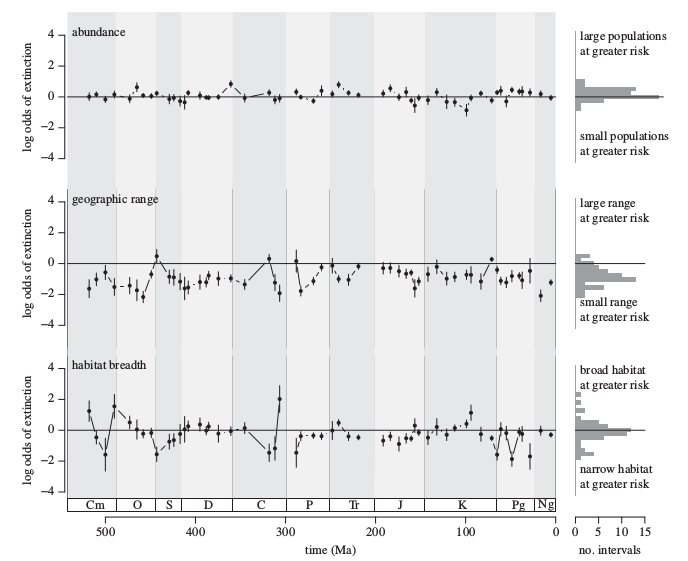
\includegraphics[width = \textwidth,height = 0.8\textheight,keepaspectratio = true]{figure/harnik_rarity}
  \end{center}
  
  \tiny{\attrib{Harnik and Simpson 2013 \textit{Proc B}}}
\end{frame}

\begin{frame}
  \frametitle{Survival of the unspecialized}
  \begin{quote}
    When related phyla die out \dots more specialized phyla tend to become extinct before less specialized. This phenomenon is also far from universal, but it is so common that it does deserve recognition as a rule or principle in evolutionary studies: \textbf{the rule of the survival of the relatively unspecialized.}

    \small{\attrib{Simpson, 1944, \em{Tempo and Mode of Evolution}, p. 143}}
  \end{quote}
\end{frame}

\begin{frame}
  \frametitle{Hypotheses of effect of environmental preference}
  % Miller and Foote
\end{frame}

\begin{frame}
  \frametitle{Hierarchical Bayesian modeling approach}

  
\includegraphics[width = \textwidth,height = 0.8\textheight,keepaspectratio = true]{figure/han_bayes}

  \tiny{\attrib{www.countbayesie.com}}
\end{frame}

\begin{frame}
  \frametitle{Hierarchical survival model}
  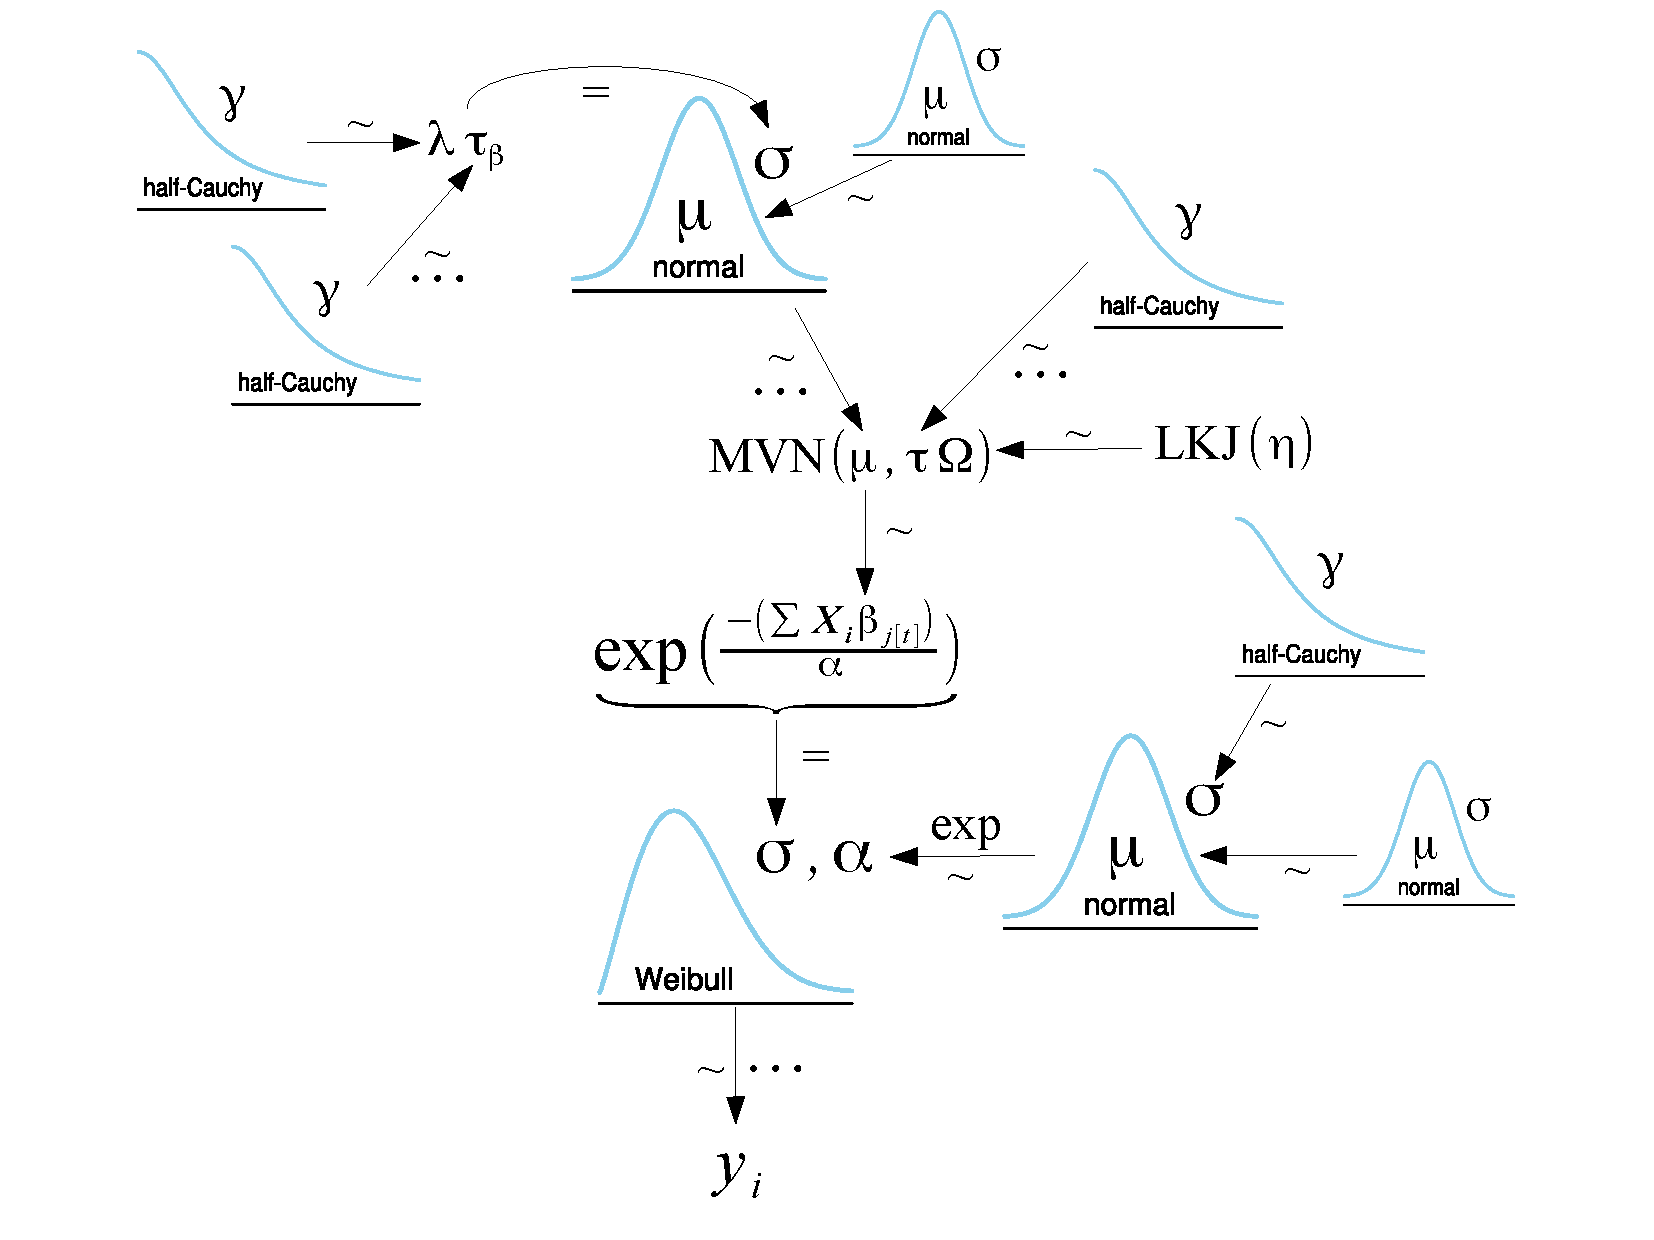
\includegraphics[width = \textwidth,height = 0.8\textheight,keepaspectratio = true]{figure/brac_surv_model}
\end{frame}

\begin{frame}
  \frametitle{Refresher on probability}

  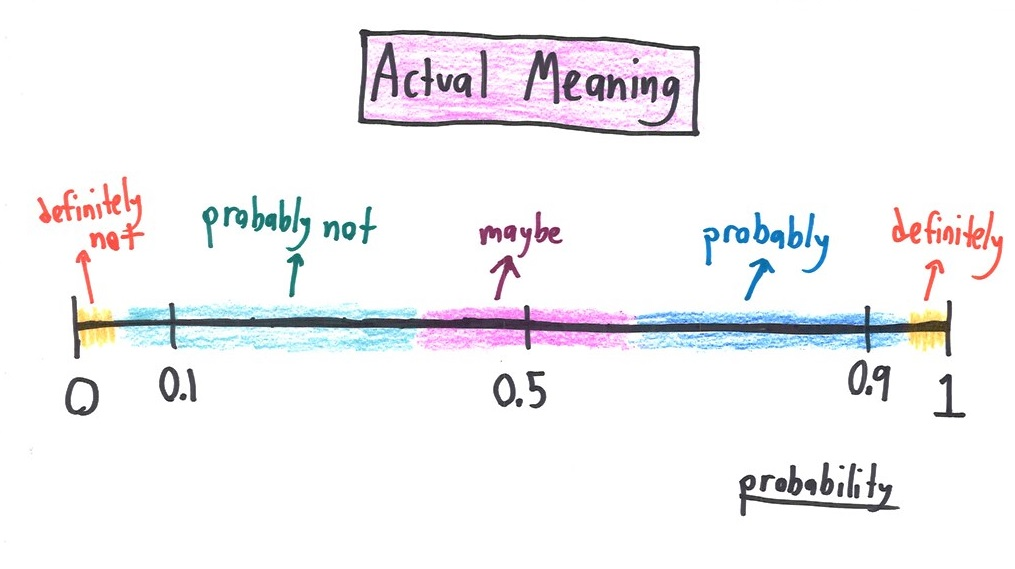
\includegraphics[width = \textwidth,height = 0.8\textheight,keepaspectratio = true]{figure/probability}

  \tiny{\attrib{www.mathwithbaddrawings.com}}
\end{frame}


\begin{frame}
  \frametitle{Posterior predictive distribution of S(t)}
  
  \begin{center}
    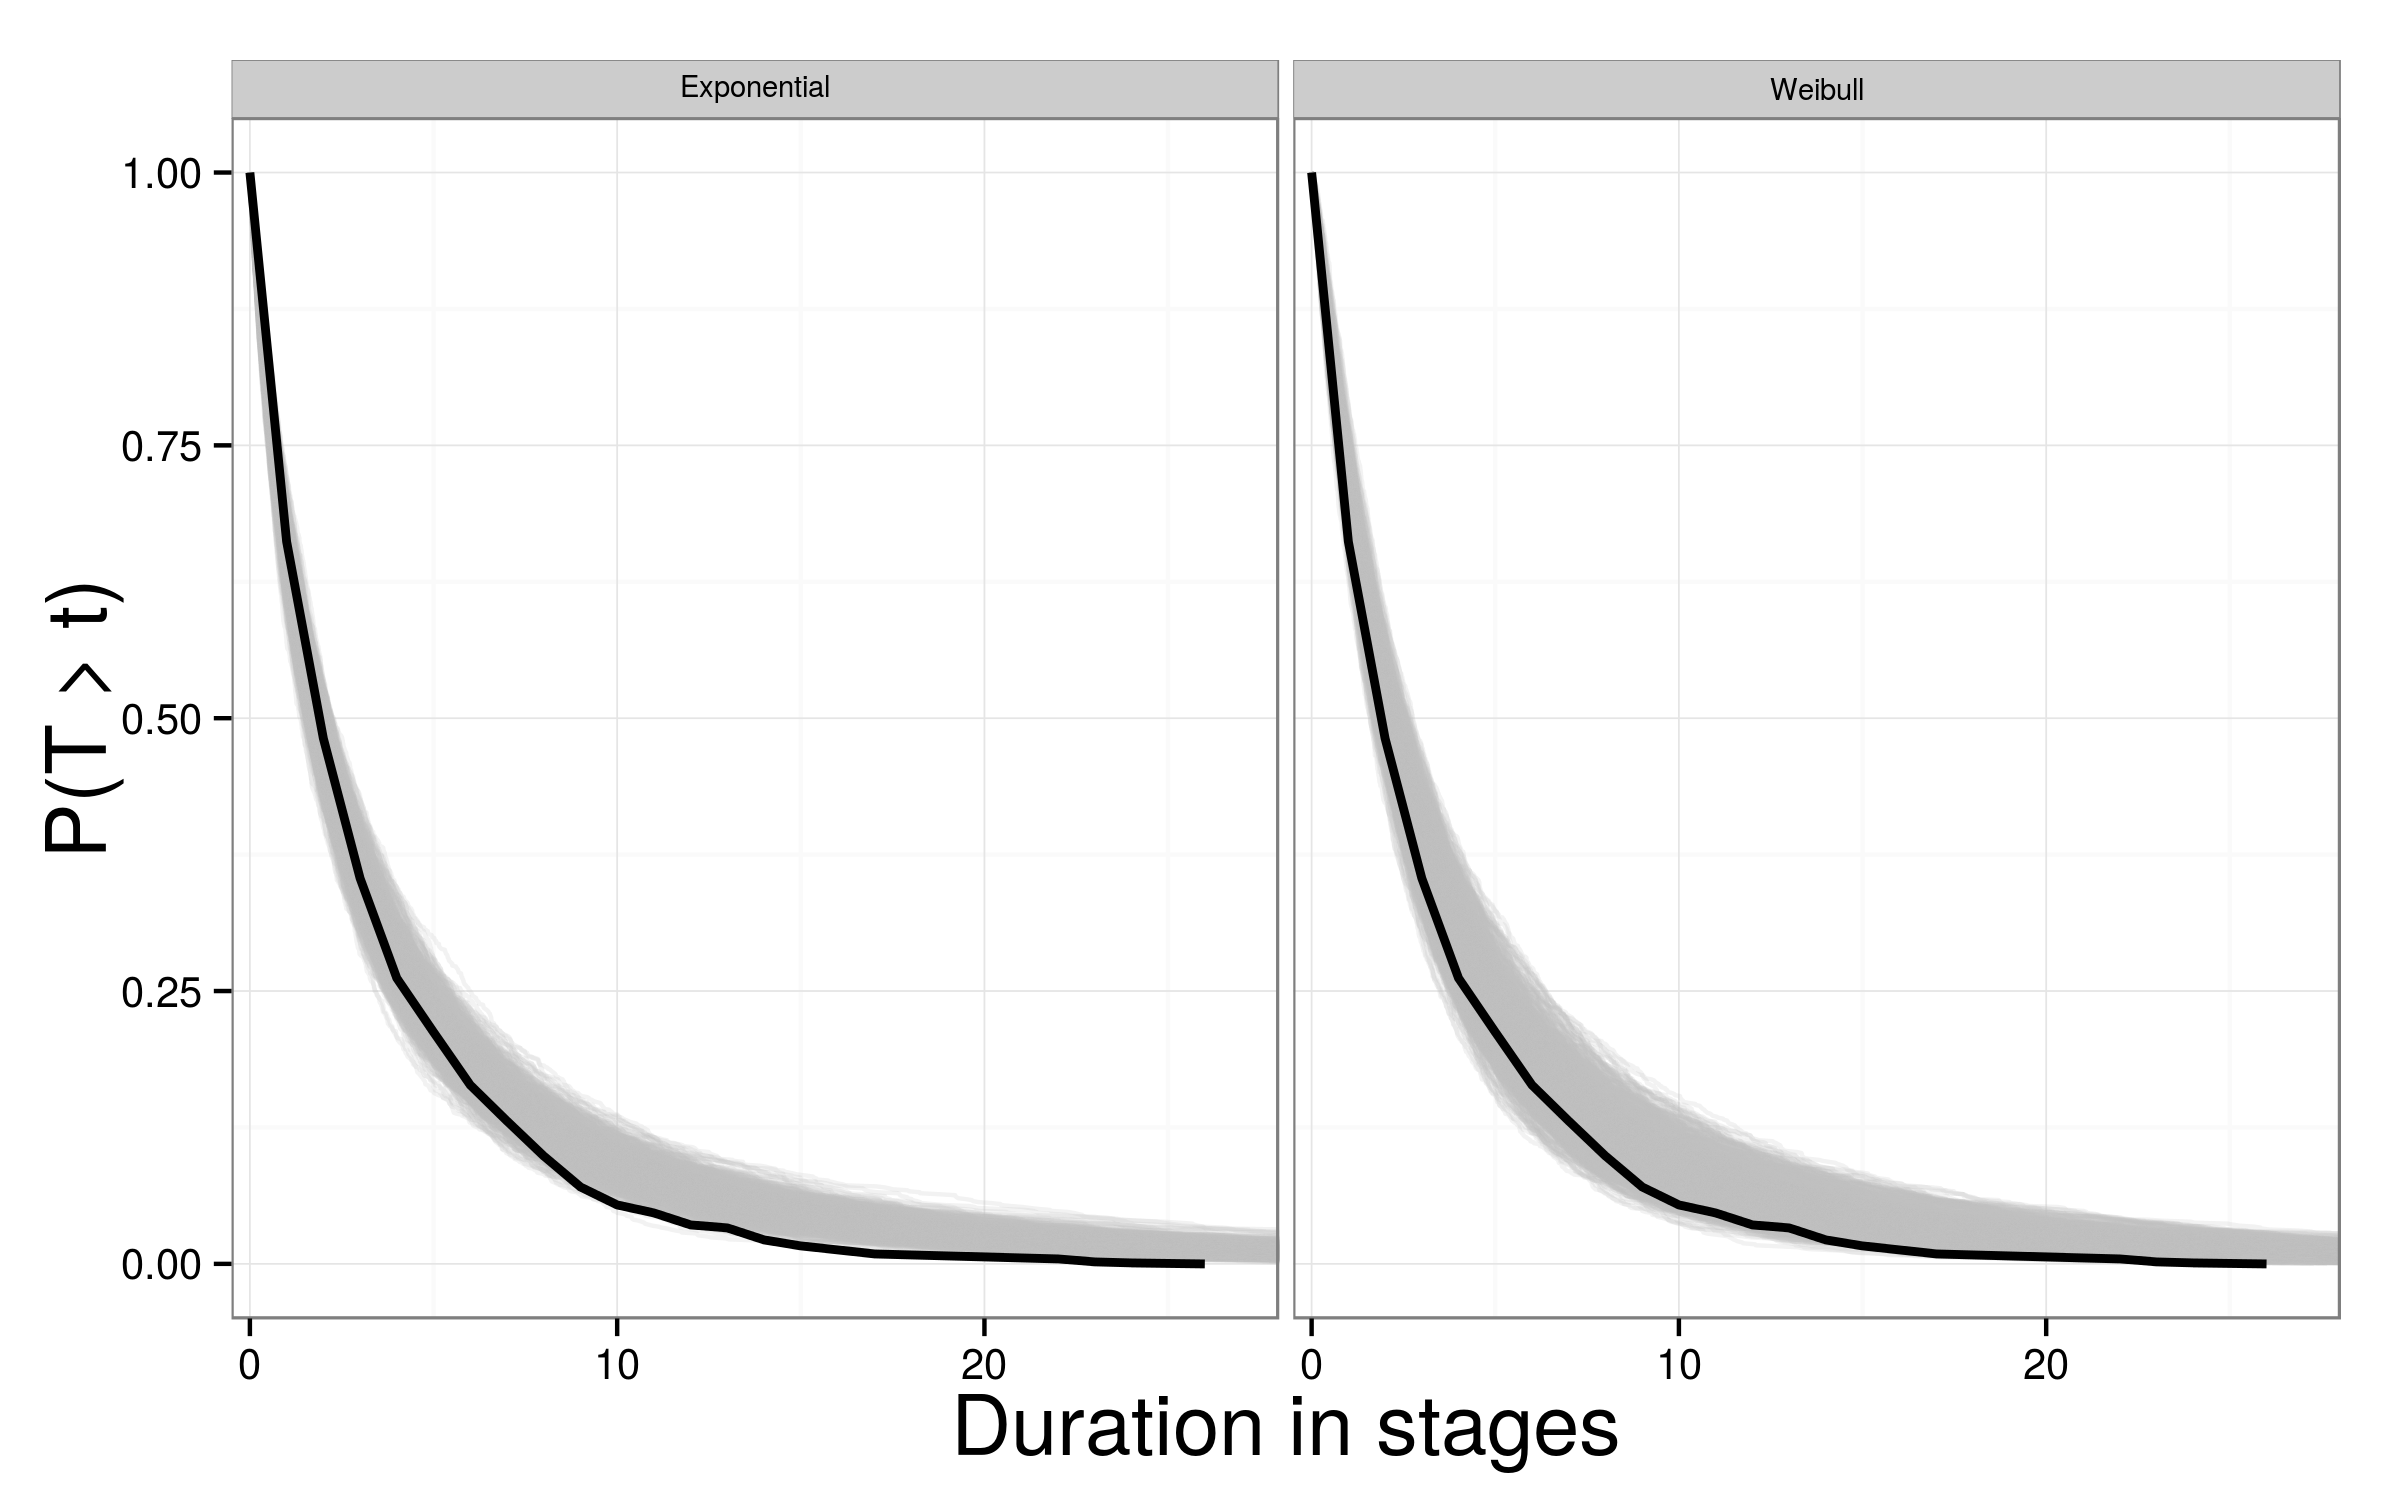
\includegraphics[width = \textwidth,height = 0.8\textheight,keepaspectratio = true]{figure/survival_curves}
  \end{center}
\end{frame}

\begin{frame}
  \frametitle{Overall effect of environmental preference}
  
  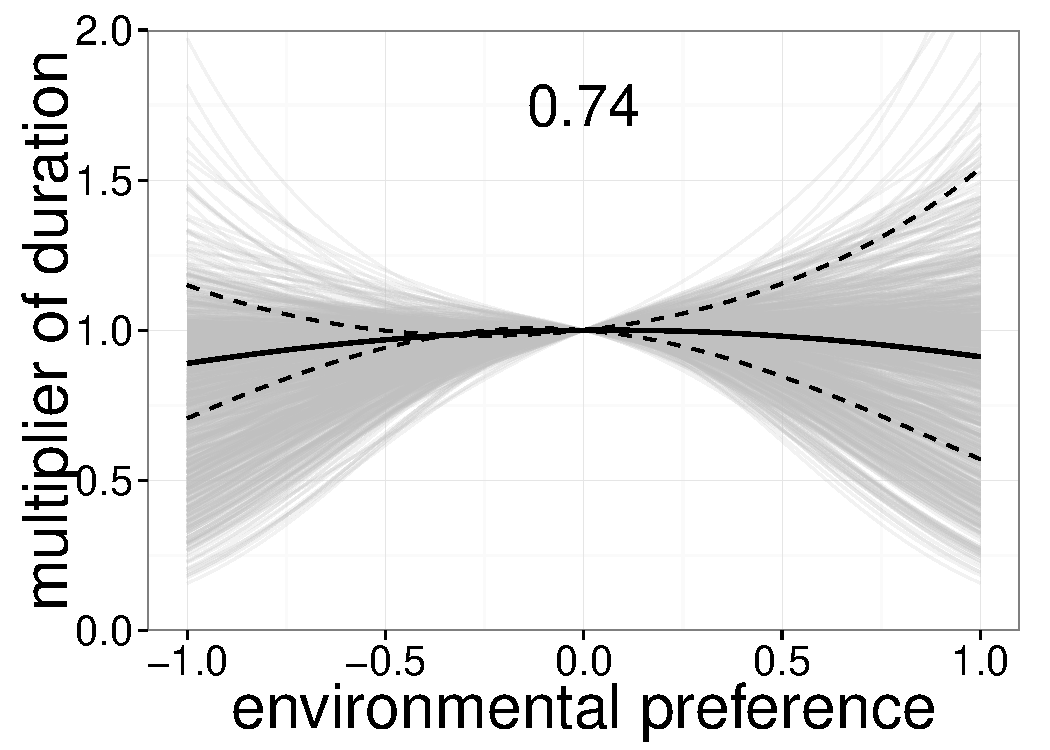
\includegraphics[width = \textwidth,height = 0.8\textheight,keepaspectratio = true]{figure/environ_quad}
\end{frame}

\begin{frame}
  \frametitle{Change in trait effects between cohorts}
  
  \begin{center}
    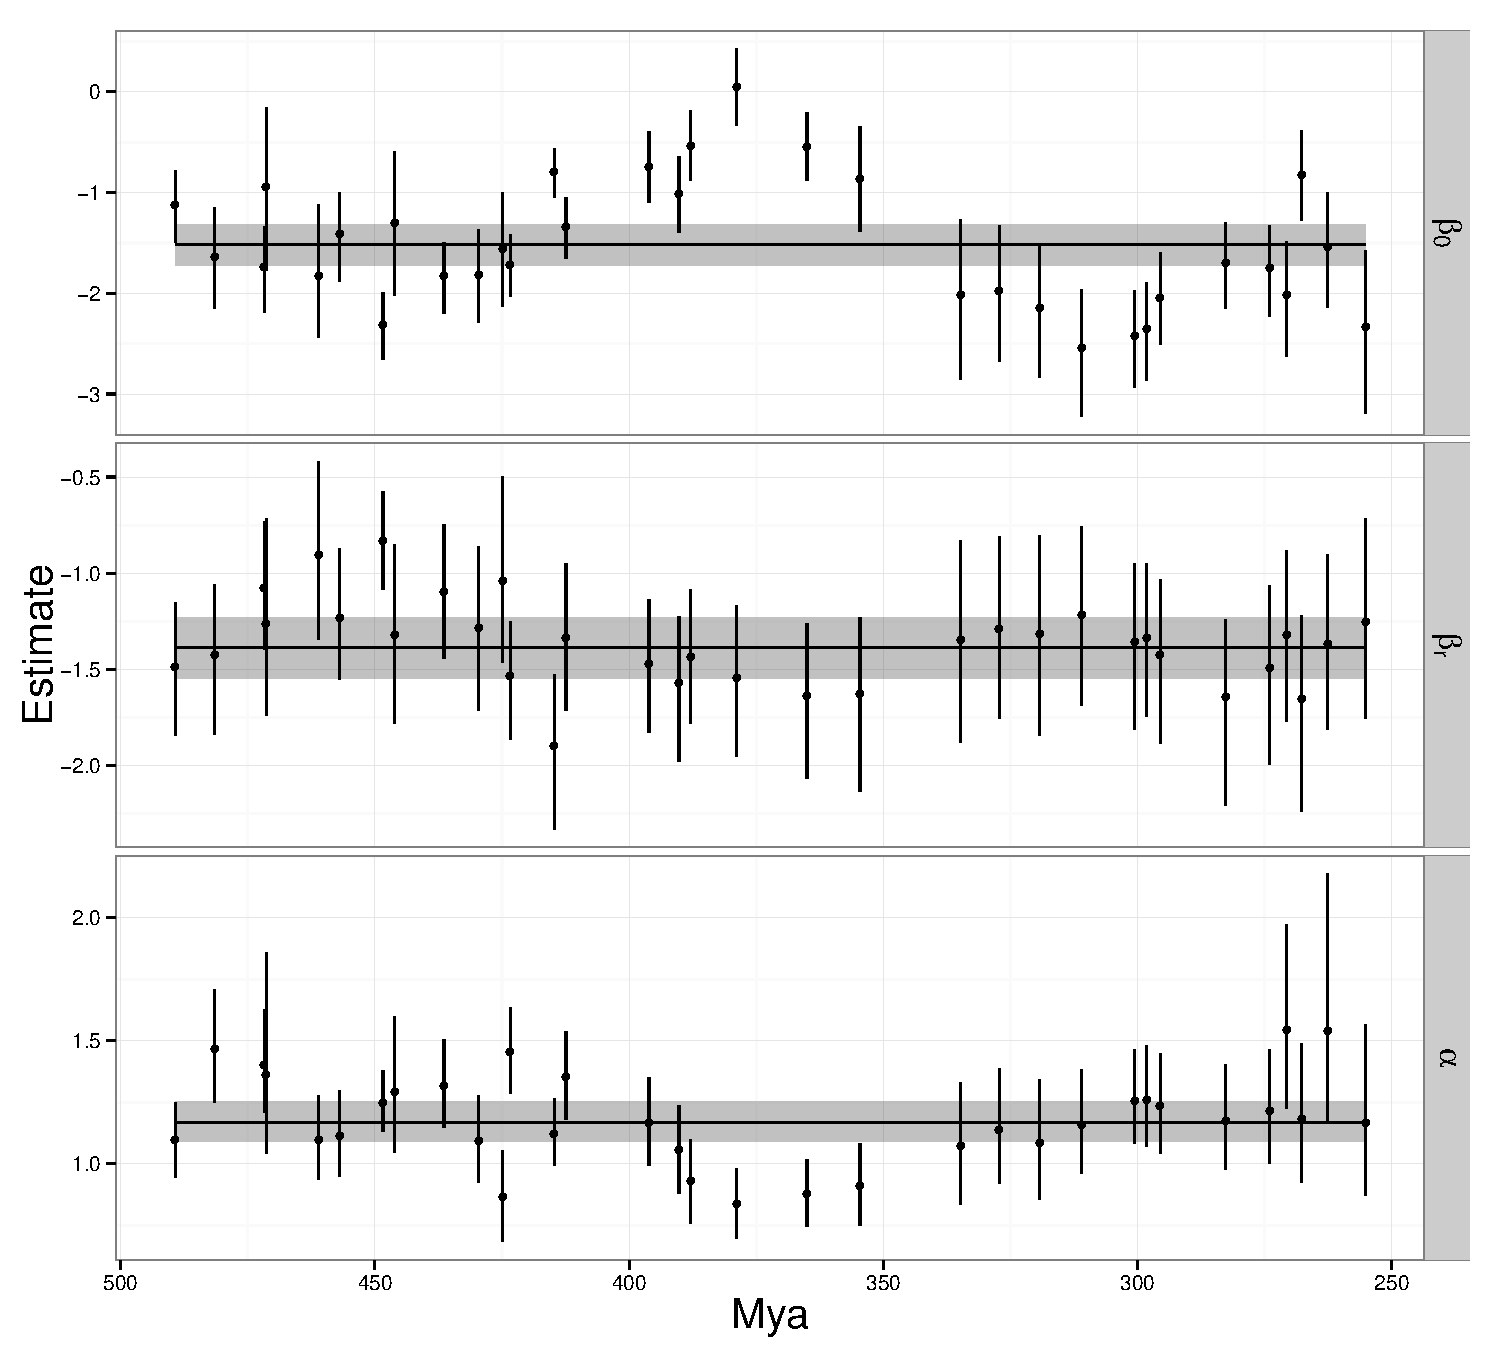
\includegraphics[width = \textwidth,height = 0.8\textheight,keepaspectratio = true]{figure/cohort_series}
  \end{center}
\end{frame}

\begin{frame}
  \frametitle{Change in effect of environment between cohorts}
  
  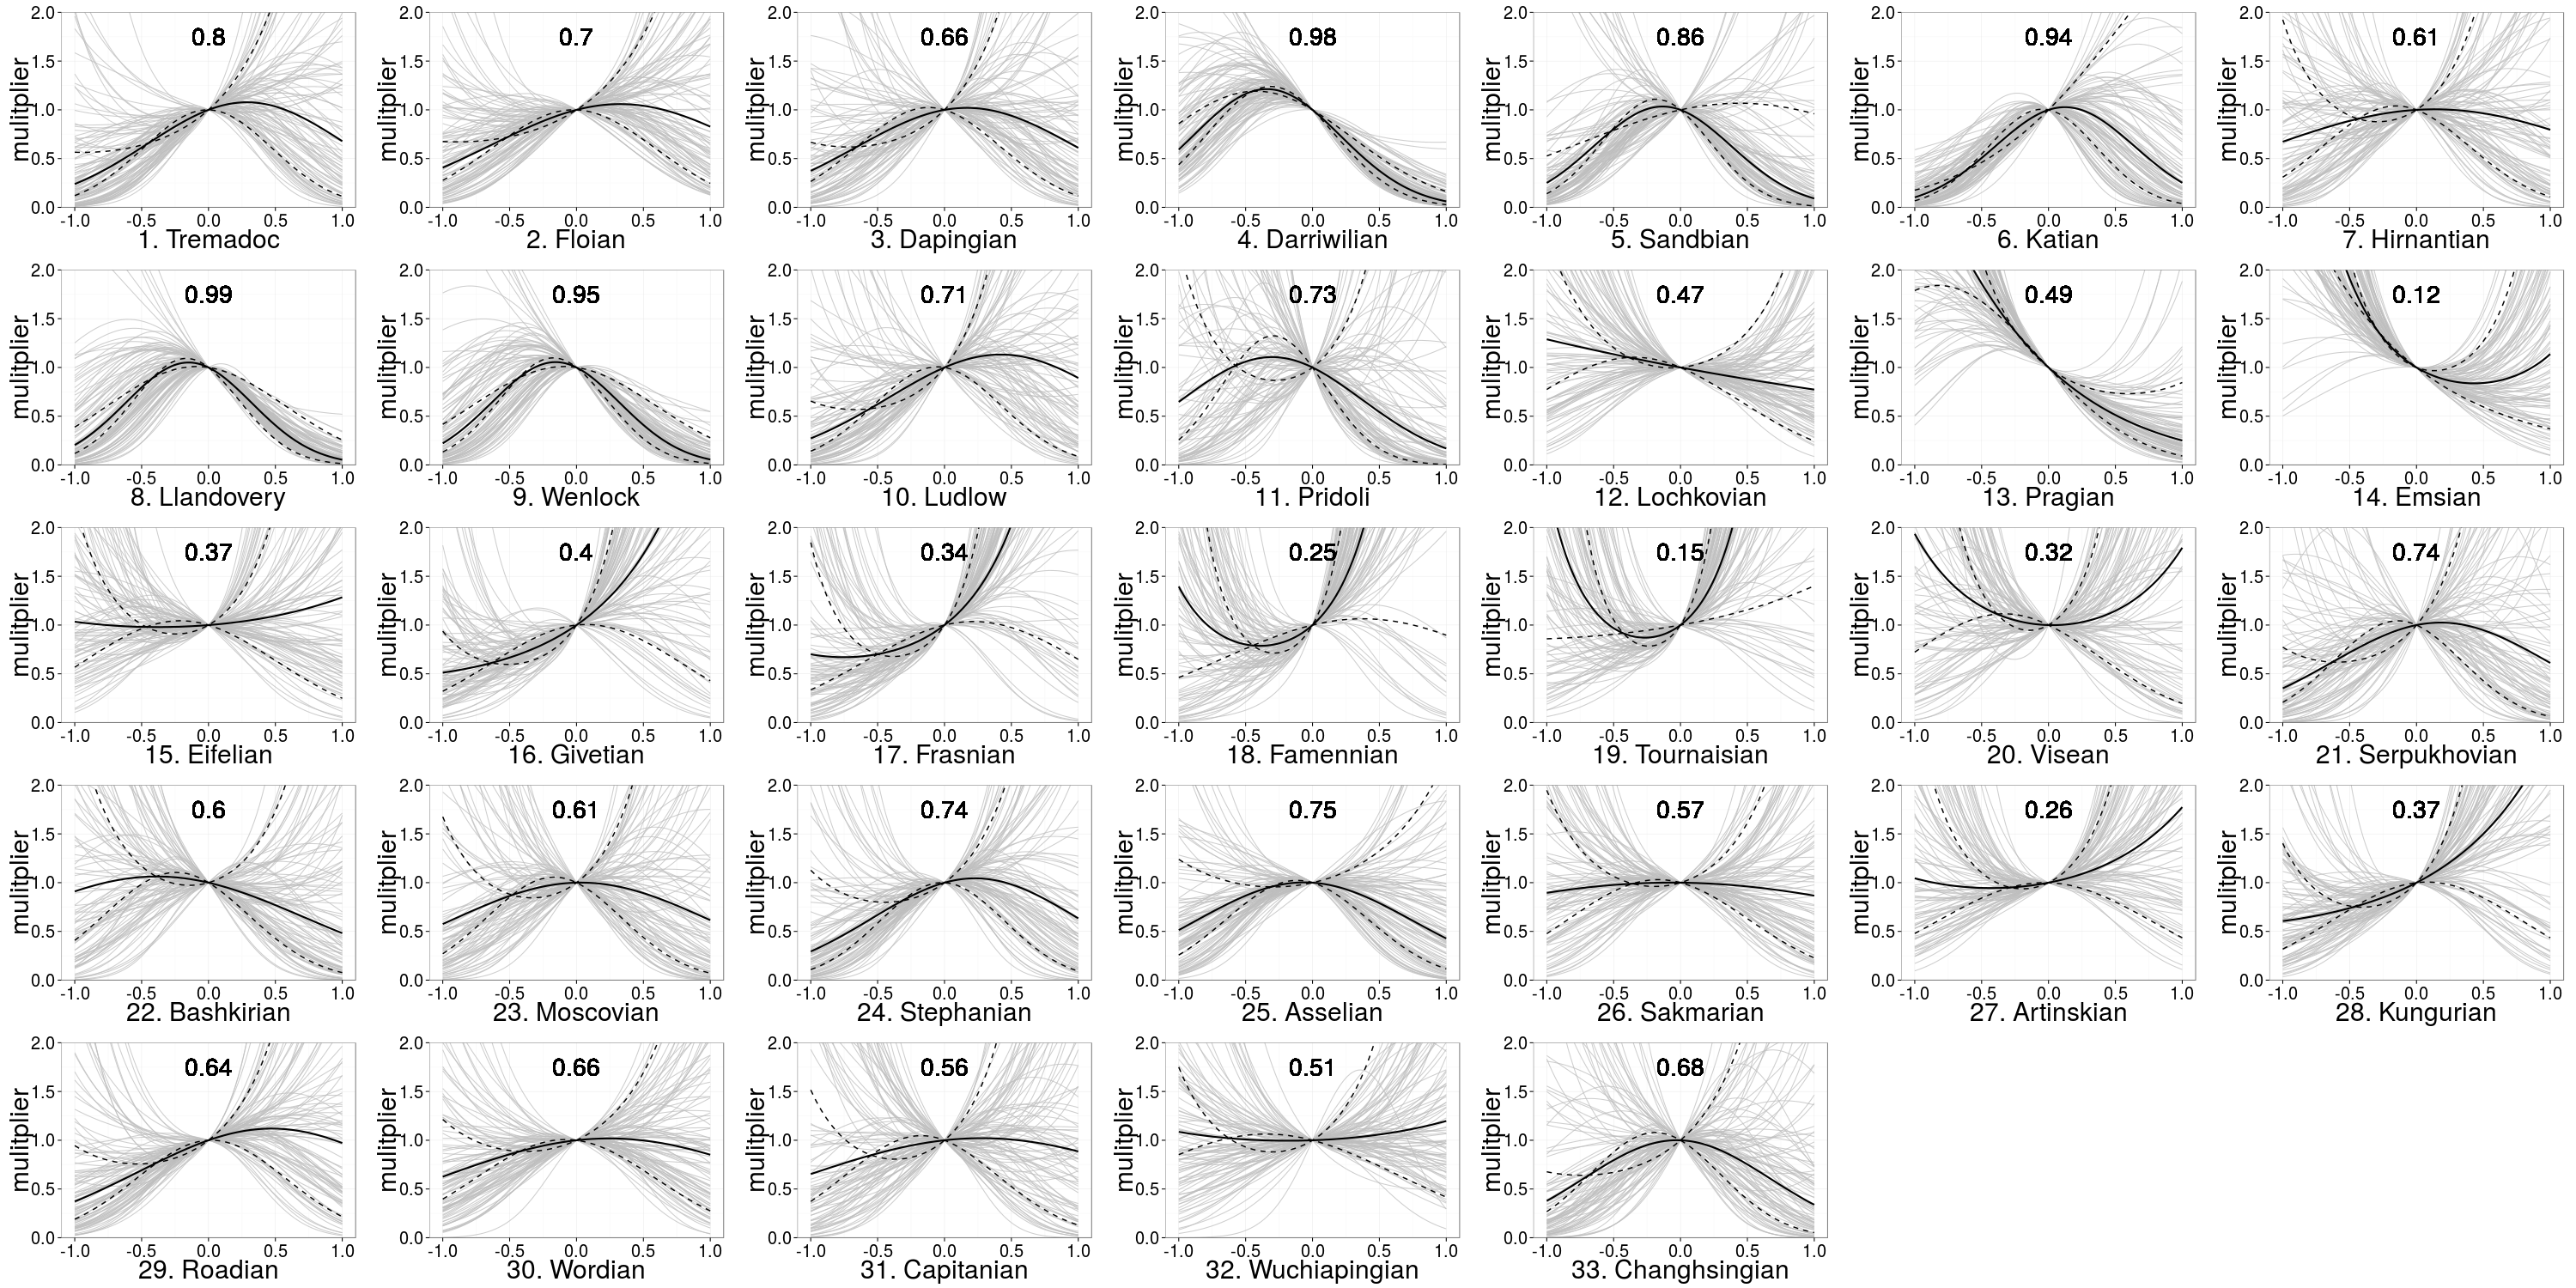
\includegraphics[width = \textwidth,height = \textheight,keepaspectratio = true]{figure/cohort_quads}
\end{frame}


\begin{frame}
  \frametitle{Correlation of effects between cohorts}
  
  \begin{center}
    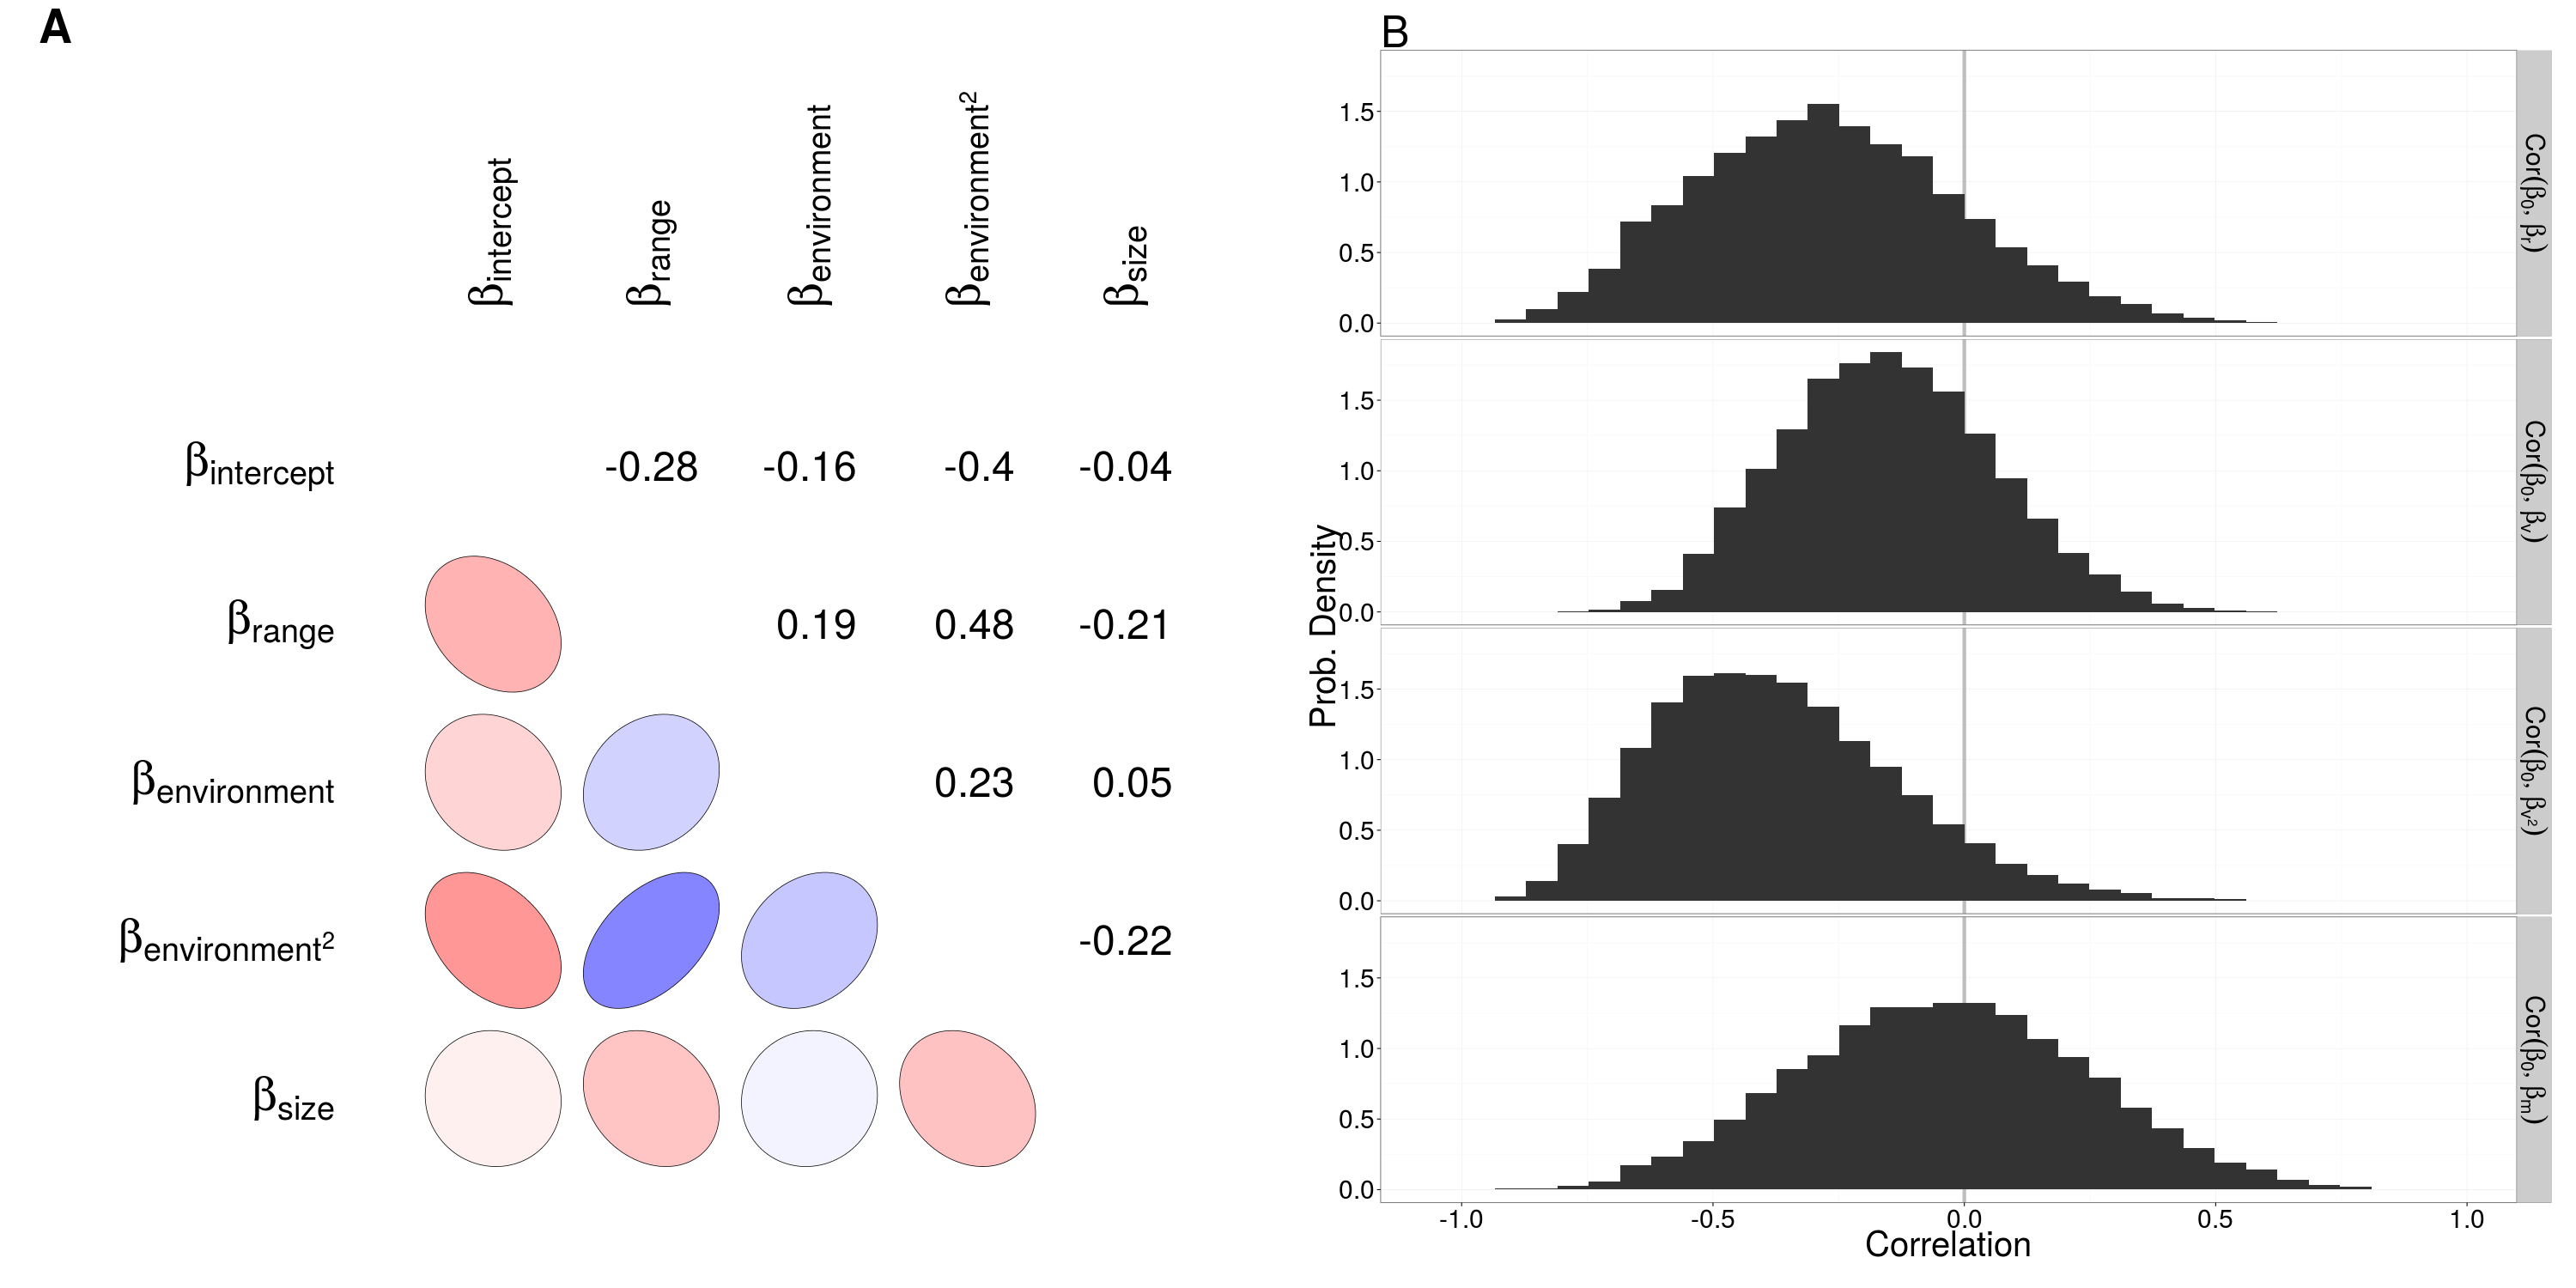
\includegraphics[width = \textwidth,height = 0.9\textheight,keepaspectratio = true]{figure/cor_mixed}
  \end{center}
\end{frame}


\begin{frame}
  \frametitle{Conclusions}
\end{frame}


\begin{frame}
  \frametitle{Acknowledgements}
  \begin{columns}
    \begin{column}{0.5\textwidth}
      \begin{itemize}
        \item Advising
          \begin{itemize}
            \item Kenneth D. Angielczyk, Michael J. Foote, \\P. David Polly, \\Richard H. Ree
          \end{itemize}
        \item Angielczyk Lab
          \begin{itemize}
            \item {\small{David Grossnickle, \\Dallas Krentzel}}
          \end{itemize}
        \item Foote lab
          \begin{itemize}
            \item {\small{Marites Villarosa Garcia, \\Nadia Pierrehumbert, \\Kathleen Ritterbush}}
          \end{itemize}
      \end{itemize}
    \end{column}
    \begin{column}{0.5\textwidth}
      \begin{itemize}
        \item {\footnotesize{Stewart Edie, \\Colin Kyle, \\Darcy Ross, \\Elizabeth Sander, \\Laura Southcott, \\Courtney Stepien}}
        \item {\footnotesize{John Alroy, \\David Bapst, \\Ben Frable, \\Graeme Lloyd, \\\textbf{Arnold Miller}, \\Carl Simpson, \\Graham Slater, \\Peter Wagner}}
      \end{itemize}
    \end{column}
  \end{columns}
\end{frame}

\appendix

\end{document}

